\subsection{Drivhus styring}

Til drivhus styring er der valgt, at bruge en Siemens LOGO! 12/24RCE. 
Den er valgt ud fra at den har indbygget 0 - 10 V input, 
som gør det muligt at tilslutte et potentiometer med en flyder på, 
så vandniveauet kan måles.
Denne LOGO! enhed har også relæ udgange, 
hvilket gør det muligt at styre flere forskellige spænding niveauer.
Så er det også muligt, at udvide med forskellige 24 V moduler, hvilket ikke er mulig i 230 V versionen.

\subsubsection{Analog indgange}
på side 41 i \cite{logo_sm} og side 42 i \cite{logo_sm} står der omkring modstande til spændingsdeling i LOGO!

\subsubsection{Luftfugtighed}
\url{http://old.gyproc.dk/files/Gyproc/Library/Handbook/DK/HB9%20-%204.5.2%20-%20Fugt%20i%20luft.pdf}
\url{http://www.vitavia.dk/filarkiv/pdf/Vitavia_broc_2017_DK_low.pdf}

Tomat i drivhus uden varme er fra omkring 1. maj
Agurk i drivhus uden varme og som små planter i slutningen af maj til juni.

Begge planter kan ikke klar temperature over 30 grader celcius.

Luftfugtighed ønskes til at være omkring.

Reduktion af Luftfugtighed kan ske via ventilation. \url{http://pure.au.dk/portal/files/42028244/743458.pdf}
Luftfugtighed agurk: 2 g kg$^{-1}$ 
Luftfugtighed tomat: 3 g kg$^{-1}$ 
80 \% RH

\url{https://www.havenyt.dk/spoergsmaal/drivhuset/12188.html}
Tomater: 20 grader om dagen
Agurk: 26 - 28 grader om dagen
\url{https://voresvilla.dk/haven/drivhus-orangeri/undga-sygdomme-drivhuset/}
Op til 4 liter vand om dagen.
\begin{figure}[!h]
    \begin{center}
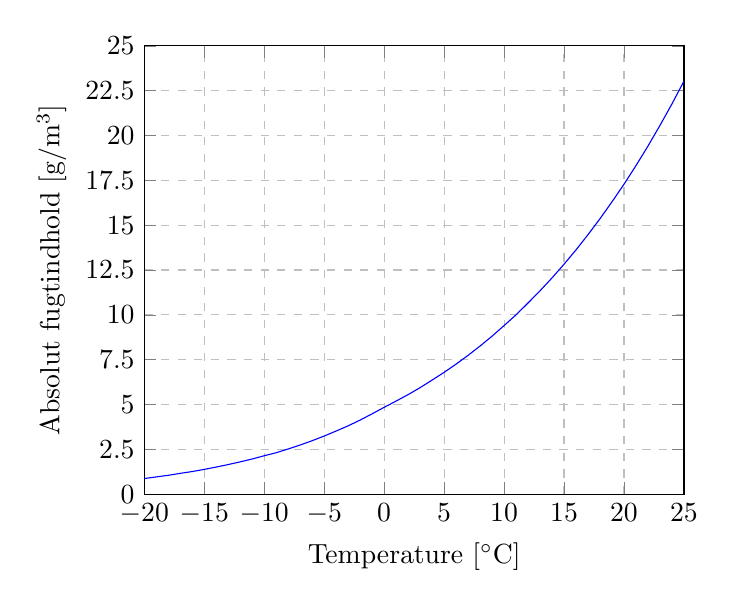
\begin{tikzpicture}
\begin{axis}[
    %title={Luft mættet med vanddamp},
    xlabel={Temperature [$^{\circ}$C]},
    ylabel={Absolut fugtindhold [g/m$^3$]},
    xmin=-20, xmax=25,
    ymin=0, ymax=25,
    xtick={-20, -15, -10, -5, 0, 5, 10, 15, 20, 25},
    ytick={0.0, 2.5, 5.0, 7.5, 10.0, 12.5, 15.0, 17.5, 20.0, 22.5, 25.0},
    %legend pos=north west,
    ymajorgrids=true,
    xmajorgrids=true,
    grid style=dashed,
]
\addplot[
    color=blue,
    mark=dot,
    ]
    coordinates {
        (-20,0.87)
        (-19,0.96)
        (-18,1.05)
        (-17,1.16)
        (-16,1.26)
        (-15,1.38)
        (-14,1.51)
        (-13,1.65)
        (-12,1.80)
        (-11,1.96)
        (-10,2.14)
        (-9,2.31)
        (-8,2.52)
        (-7,2.74)
        (-6,2.98)
        (-5,3.24)
        (-4,3.52)
        (-3,3.81)
        (-2,4.13)
        (-1,4.48)
        (0,4.84)
        (1,5.19)
        (2,5.55)
        (3,5.94)
        (4,6.36)
        (5,6.79)
        (6,7.25)
        (7,7.74)
        (8,8.26)
        (9,8.81)
        (10,9.40)
        (11,10.00)
        (12,10.66)
        (13,11.34)
        (14,12.06)
        (15,12.82)
        (16,13.62)
        (17,14.47)
        (18,15.36)
        (19,16.30)
        (20,17.28)
        (21,18.32)
        (22,19.41)
        (23,20.56)
        (24,21.76)
        (25,23.03)        
    };
    %\legend{g/m$^3$}
\end{axis}
\end{tikzpicture}
\end{center}
\caption{Luft mættet med vanddamp}\label{fig:luft_vanddamp}
\end{figure}